\newpage
	\flushright{\hyperref[index]{\color{black!65}{Ritorna all'indice}}}\flushleft
	\section{P} \label{sec:P}
	
		\subsection{3P}	\index{3P}	\label{3p}
		Stanno per: \textit{Product}, \textit{Process}, \textit{Progression in learning} (e Incrementalmente). Sono i 3 (4) punti di avanzamento chiave del progetto. Le 3P sono la \textit{capstone}(=parte finale di una struttura) project.
		
		\subsection{PIANIFICAZIONE} \index{Pianificazione} \label{pianificazione}
		Definisce delle attività al fine di pianificarne lo svolgimento e controllarne l’attuazione, avere una base su cui gestire l’allocazione delle risorse e per stimare e controllare scadenze e costi. Per la pianificazione vengono utilizzati degli \textit{strumenti} quali: \underline{\hyperref[gantt]{Diagramma di Gantt}}, \underline{\hyperref[pert]{PERT}} e \underline{\hyperref[wbs]{WBS}}. \\		
		In breve: chi fa cosa - quando - in quanto tempo - quanto costa. 
	
		\subsection{PIANO DI PROGETTO} \index{Piano di progetto} \label{piano}
		Il piano di progetto (o \textit{PdP}) sostanzialmente è un documento ufficiale, soggetto ad approvazioni, con il quale si descrivono gli obiettivi di progetto e gli elementi necessari per il loro raggiungimento. Si vedono le risorse disponibili e le loro assegnazioni alle attività con scansione delle attività nel tempo. L'attività più importante è l'analisi dei rischi. \\
		Principalmente è scomposto in:
			\begin{itemize}
				\item Pianificazione(preventiva)
					\begin{itemize}
						\item team;
						\item \underline{\hyperref[analisirischi]{analisi dei rischi}};
					\end{itemize}
				\item \underline{\hyperref[consuntivo]{Consuntivazione}}: è lo specchio della pianificazione. Fa una valutazione retrospettiva;
			\end{itemize}
		Tipicamente la struttura del PdP è composta da:
			\begin{itemize}
				\item Introduzione (scopo e struttura);
				\item Organizzazione del progetto;
				\item \underline{\hyperref[analisirischi]{Analisi dei rischi}};
				\item Risorse disponibili (tempo e persone);
				\item Suddivisione del lavoro (work breakdown);
				\item Calendario delle attività (project schedule);
				\item Meccanismo di controllo e di rendicontazione;
			\end{itemize}
		È da tenere presente che ci sono anche dei rischi di progetto, quali sforamento di costi o tempi, che derivano da fonti come tecnologie di lavoro e produzione, rapporti interpersonali, organizzazione del lavoro, rapporti con gli stakeholder e appunto tempi e costi. Per questo ci vuole una \underline{\hyperref[gestionerischi]{Gestione dei rischi}}. 
		
		%Quali contenuti:
		%Quale struttura:
		
		\subsection{PIANO DI QUALIFICA}	\index{Piano di Qualifica}	\label{pianoqualifica}
		Definisce le strategie di \underline{\hyperref[verificare]{verifica}} e \underline{\hyperref[validare]{validazione}} (metodi, tecniche, procedure, strumenti e tempi). Per ogni passo fatto in analisi o altro, preparare i test e fare il tracciamento per non perdere nulla, per dare qualità (consultare \underline{\hyperref[V]{modello a V}}); questo documento specifica quali e quante prove effettuare. Anche questo documento, come le \underline{\hyperref[norme]{Norme}}, è incrementale. \\
		Si parla qui di metriche e obiettivi di "oggi" (ad esempio requisiti, fluttuazione requisiti). \\
		\textbf{N.B:} le metriche vanno inserite nelle Norme (vedere correzione Breaking Bug) mentre gli obiettivi nel PdQ.
		
		\subsection{PIANO DI QUALITÀ}	\index{Piano di Qualià}	\label{pianoqualita} %slide 8/22 Set Qualità del software
		Attività del sistema qualità mirate a fissare gli obiettivi di \underline{\hyperref[qualita]{qualità}}, e i processi e le risorse necessarie per conseguirli. \\
		Stabilisce qual è il modo in cui noi perseguiamo la qualità. Si fissano le politiche aziendali e si determinano gli obiettivo di qualità del singolo progetto.
		
		\subsection{PORTABILITÀ}	\index{Portabilità}	\label{portabilita}
		Un prodotto che ha la proprietà di adattarsi ad altri dispositivi.
		  		 
		\subsection{PREVENTIVO} \index{Preventivo} \label{preventivo}
		Stima iniziale dei costi necessari alla realizzazione di un \underline{\hyperref[progetto]{progetto}}. (PAF = preventivo a finire, da attuarsi in corso d'opera perché diventa sempre più preciso).
	
		\subsection{PRINCIPIO DEL MIGLIORAMENTO CONTINUO} \index{Principio del miglioramento continuo} \label{miglioramentocontinuo}
		Identifica specifici obiettivi di miglioramento, li esegue, ne verifica l'esito e infine agisce sulle conseguenze (per esempio, se considerato buono, lo tiene nello standard).
		
		\subsection{PROBLEM RESOLUTION}	\index{Problem solution}	\label{problemsolution}
		Avere un metodo molto chiaro non violabile per la soluzione di problemi. È di \underline{\hyperref[12207]{ISO 12207}}. \\
		È fatto di una strategia nota (il nostro way of working). In essa tutti i problemi sorti sono stati registrati e ogni problema va studiato individualmente decidendo quali soluzioni sono accettabili. Viene in seguito realizzata la soluzione scelta e verificato l'esito della correzione. % slide 10/22
		È comunque un'azione correttiva e non buona [da inserire nel ticketing] fatta tramite \underline{\hyperref[testregressione]{Test di regressione}}.
		
		\subsection{PROCESSO} \index{Processo} \label{processo}
		Insieme di attività \underline{\hyperref[correlato]{correlate}} e \underline{\hyperref[coeso]{coese}} che trasformano bisogni in \underline{\hyperref[prodotto]{prodotti}}. Opera secondo regole e nel farlo consuma risorse. Questo insieme di attività (tra cui la \underline{\hyperref[gestioneprogetto]{Gestione di Progetto}}) deve essere \underline{\hyperref[efficienza]{efficiente}} ed \underline{\hyperref[efficacia]{efficace}}. Adottare \underline{\hyperref[standard]{standard}} di processo aiuta a raggiungere l'\underline{\hyperref[economicita]{economicità}}.\\
		Tra le \textit{attività di processo} per lo sviluppo software troviamo: 
			\begin{enumerate}
				\item \textbf{Istanziazione del processo};
				\item \textbf{Analisi dei requisiti del sistema};
				\item \textbf{Progettazione architetturale del sistema};
				\item \textbf{\underline{\hyperref[analisideirequisiti]{Analisi dei requisiti}} del SW};
				\item \textbf{\underline{\hyperref[progettazione]{Progettazione}} architetturale del SW};
				\item \textbf{Progettazione di dettaglio del SW};
				\item \textbf{Codifica e prova delle componenti SW}: comprende i compiti
					\begin{itemize}
						\item Definire procedure e dati di prova;
						\item Eseguire e documentare le prove;
						\item Aggiornare documentazione e pianificare prove d’integrazione;
						\item Valutare l’esito delle prove;
					\end{itemize}
				\item \textbf{Integrazione delle componenti SW}: comprende i compiti
					\begin{itemize}
						\item Definire il piano di integrazione;
						\item Eseguire e documentare le prove;
						\item Aggiornare documentazione e pianificare prove di collaudo;
						\item Valutare l’esito delle prove;
					\end{itemize}
				\item \textbf{Collaudo del SW}: comprende i compiti
					\begin{itemize}
						\item Eseguire e documentare il collaudo;
						\item Valutare l’esito del collaudo;
					\end{itemize}	
				\item \textbf{Integrazione di sistema}: comprende i compiti
					\begin{itemize}
						\item Eseguire e documentare le prove;
						\item Aggiornare documentazione e pianificare prove di collaudo;
						\item Valutare l’esito delle prove;
					\end{itemize}
				\item \textbf{Collaudo del sistema}: comprende i compiti
					\begin{itemize}
						\item Eseguire e documentare il collaudo;
						\item Valutare l’esito del collaudo;
					\end{itemize}
			\end{enumerate}
		L'adozione di processi deve essere consapevole ed \underline{\hyperref[efficacia]{efficace}}, per questo ci deve essere una buona \textit{organizzazione}:
			\begin{itemize}
				\item \textbf{Processo standard} è il riferimento di base generico ed è condiviso tra diverse aziende nello stesso dominio applicativo.
				\item \textbf{Processo definito} è una specializzazione del processo standard al fine di adattarlo a specifiche esigenze. Tra i processi definiti troviamo i \textbf{processi specializzati per azienda} che sono chiari, stabili, documentati, indipendenti dal modello di \underline{\hyperref[ciclo]{ciclo di vita}} adottato, dalle tecnologie, dal dominio applicativo e dalla documentazione richiesta.
				\item \textbf{Processo di progetto} è un'istanziazione di processi definiti che utilizzano risorse aziendali per raggiungere obiettivi prefissati e con scadenze (progetti). I processi specializzati per progetto sono ben pianificati, hanno chiare scelte di specializzazione (definire lo scenario di applicazione e le attività, organizzare le relazioni tra processi) e l'esito viene valutato in maniera critica.
			\end{itemize}
		L'organizzazione interna dei processi, per essere buona, deve inoltre essere incentrata sul principio di miglioramento continuo: il \underline{\hyperref[pdca]{ciclo di Deming}}.
			
		Per quel che riguarda la specializzazione di processi, abbiamo dei \textit{fattori di specializzazione} che c'entrano con: la dimensione e la complessità del \underline{\hyperref[progetto]{progetto}}, i rischi (come dominio applicativo e tecnologie in uso), la competenza delle risorse umane e i fattori dipendenti dal contratto.\\
		\textit{Fattori di influenza}:
			\begin{itemize}
				\item I processi non determinano quale \underline{\hyperref[ciclo]{ciclo di vita}}, ma al contrario, il ciclo di vita determina quali processi attivare;
				\item Il livello di coinvolgimento del cliente determina le revisioni necessarie e l'intensità della documentazione;
				\item Il \underline{\hyperref[ciclo]{ciclo di vita}} viene scelto in base a cosa vuole il \underline{\hyperref[committente]{committente}} (se versione unica non modificabile o versione destinata a continue evoluzioni) e al tipo di coinvolgimento del committente nell'accertamento dello \underline{\hyperref[stato]{stato}} di avanzamento (se revisioni interne o esterne, bloccanti o non bloccanti);
			\end{itemize}
		
		\subsection{PRODOTTO SOFTWARE} \index{Prodotto software} \label{prodotto}
		Software progettato per essere rilasciato all'utente. Viene visto come insieme di parti (che hanno a che vedere con forma, contenuto e funzione) organizzate secondo una \underline{\hyperref[configurazione]{configurazione}} per ragioni di convenienza e semplicità. La forma che ha dipende dalla richiesta. Può essere
			\begin{itemize}
				\item \textbf{commessa} se le parti vengono fissate del committente;
				\item \textbf{pacchetto} se le parti sono idonee alla replicazione;
				\item \textbf{componente} se le parti sono adatte alla composizione;
				\item \textbf{servizio} se le parti sono fissate dal problema;
			\end{itemize}
		Gli stati principali di un prodotto SW sono: concezione, sviluppo, utilizzo, ritiro [noi ci concentriamo sullo sviluppo, per questo parliamo di modelli di sviluppo].
		Il suo comportamento viene delineato dal \underline{\hyperref[ciclo]{ciclo di vita}} che, se lungo, ha notevoli costi di \underline{\hyperref[manutenzione]{manutenzione}}. 
		Il prodotto deve essere \textit{configuration item}, stare su una repository. \\
		%Qualunque risultato di processo si chiama prodotto. % da inserire in contesto
		Il software deve fare queste cose quantificabili:
		\begin{itemize}
			\item \textbf{COSA}: il software deve fare quei calcoli (caratteristiche funzionali);
			\item \textbf{COME}: in che modo fare quei calcoli (caratteristiche non funzionali);
		\end{itemize}
		e ciò richiede \underline{\hyperref[verificare]{verifica}}.
		
		\subsection{PRODUCT BASELINE}	\index{Product Baseline} \label{productbaseline}
		Deve esistere un prodotto, idealmente finito, e bisogna essere pronti alla validazione. Presenta la \underline{\hyperref[baseline]{baseline}} architetturale del prodotto (design patterns adottati) e va data tramite "allegato tecnico" con diagrammi delle classi e di sequenza. Parte della \underline{\hyperref[RQ]{RQ}}.
		
		\subsection{PRODUTTIVITÀ} \index{Produttività} \label{produttivita}
		Misurazione dell' \underline{\hyperref[efficienza]{efficienza}} in base alle aspettative soddisfatte.
		
		\subsection{PROGETTAZIONE} \index{Progettazione} \label{progettazione} %V.I.
		In inglese \textit{Design}. Essenzialmente si pensa ad una soluzione (\textit{Come fare la cosa giusta?}) dopo aver fatto l'\underline{\hyperref[analisideirequisiti]{Analisi dei Requisiti}} (\textit{Qual è il problema e qual è la cosa giusta da fare?}). Essa precede la \underline{\hyperref[realizzazione]{realizzazione}} perseguendo la \underline{\hyperref[correttezza]{correttezza}} per costruzione anziché la correttezza per correzione. È importante progettare per dominare la complessità del prodotto (di“\underline{\hyperref[divideetimpera]{divide-et-impera}}”), organizzare e ripartire le responsabilità di realizzazione, produrre in economia (\underline{\hyperref[efficienza]{efficienza}}) e garantire \underline{\hyperref[qualita]{qualità}} (\underline{\hyperref[efficacia]{efficacia}}). Mentre l'Analisi richiede comprensione del dominio e attua un \textit{approccio investigativo} (da uno a tanti), la progettazione ricerca una soluzione soddisfacente per tutti gli \underline{\hyperref[stakeholder]{stakeholder}}, descrive l'architettura del prodotto prima di pensare al codice e attua un \textit{approccio sintetico} (dal tanto al poco). \\
		
		Gli obiettivi della progettazione sono: 
		\begin{itemize}
			\item soddisfare i requisiti con un sistema di \underline{\hyperref[qualita]{qualità}} definendo l'\underline{\hyperref[architettura]{architettura}} logica del prodotto (impiegando parti con specifica chiara e \underline{\hyperref[coeso]{coesa}} realizzabili con risorse sostenibili e costi fissati, organizzate in modo da facilitarne cambiamenti in futuro);
			\item ricercare soluzioni architetturali utili al caso e con parti riusabili;
			\item  dominare la complessità del sistema suddividendolo in parti con complessità trattabile e in modo da essere un compito rapido e verificabile da un singolo individuo;
			\item spingere quindi la progettazione nel dettaglio ma senza arrivare al momento in cui il costo di coordinamento delle parti supera il beneficio della suddivisione; 
		\end{itemize}
	
		Progettare per riuso è difficile, come lo è anticipare i bisogni futuri, e non è immediato perchè bisogna minimizzare le modifiche alle componenti riusate affinché esse non perdano valore. Nel breve periodo il riuso è solo costo, diventa risparmio solo nel medio termine.\\
		La progettazione architetturali può seguire un approccio \underline{\hyperref[topdown]{top-down}}, \underline{\hyperref[bottomup]{bottom-up}} oppure \textit{meet-in-the-middle} che è una via di mezzo e il più frequentemente usato. Se si impone uno stile architetturale, il \textit{framework} (ha un'architettura) è top-down oltre che contemporaneamente bottom-up dato che è fatto di codice già sviluppato (esempi spring, struts, ecc).\\
		Nella progettazione si parla anche di \textit{Design pattern} architetturali: sono nati con dei principi, sono la soluzione progettuale al problema ricorrente e suggeriscono un'organizzazione architetturale con proprietà note ottenibili solo con una buona istanziazione e coerente implementazione (sono il corrispondente architetturale degli algoritmi). \\
		Gli obiettivi della progettazione di dettaglio sono:
		
		Gli stati di progresso della progettazione secondo \underline{\hyperref[semat]{SEMAT}} sono:
			\begin{itemize}
				\item underline{\hyperref[architectureselected]{Architecture selected}};
				\item underline{\hyperref[demonstrable]{Demonstrable}};	
				\item underline{\hyperref[usable]{Usable}};
				\item underline{\hyperref[ready]{Ready}};									
			\end{itemize}
		
		La progettazione di dettaglio si occupa di definire le \underline{\hyperref[unita]{unità}} realizzative in modo che il carico di lavoro sia compiuto dal singolo programmatore.
		
		
		\subsection{PROGETTISTA} \index{Progettista} \label{progettista}
		È uno dei \underline{\hyperref[ruoli]{ruoli}} in un progetto. Generalmente sono pochi e accompagnano lo sviluppo ma non la \underline{\hyperref[manutenzione]{manutenzione}}. Hanno competenze tecniche e tecnologie aggiornate, motivo per cui influiscono su quest'ultime. 
		
		\subsection{PROGETTO} \index{Progetto} \label{progetto}
		Insieme ordinato di 4 attività:
			\begin{enumerate}
				\item \underline{\hyperref[pianificazione]{\textbf{Pianificazione}}} che gestisce le risorse (come tempo, soldi, ecc..) e le responsabilità;
				\item \underline{\hyperref[analisideirequisiti]{\textbf{Analisi dei requisiti}}} che definisce \textbf{cosa} fare;
				\item \underline{\hyperref[progettazione]{\textbf{Progettazione}}} che definisce \textbf{come} fare;
				\item \underline{\hyperref[realizzazione]{\textbf{Realizzazione}}} che esegue perseguendo \underline{\hyperref[qualita]{qualità}} e fa \underline{\hyperref[verificare]{verifica}} e \underline{\hyperref[validare]{validazione}};
			\end{enumerate}	
		le quali realizzano processi di \underline{\hyperref[ciclo]{ciclo di vita}} e devono:
			\begin {itemize}
				\item raggiungere obiettivi;
				\item avere inizio e fine fissate (scadenze);
				\item avere risorse limitate;
				\item consumare le suddette risorse.
			\end {itemize}
		Nel suo complesso il progetto è sempre collaborativo. La disciplina da prendere come riferimento è l'\underline{\hyperref[swe]{Ingegneria del Software}}.\\
		L'organizzazione \underline{\hyperref[semat]{SEMAT}} definisce i principali elementi di un progetto:
			\begin{itemize}
				\item \textbf{\underline{\hyperref[customer]{customer}}};
				\item \textbf{\underline{\hyperref[solution]{solution}}};
				\item \textbf{\underline{\hyperref[endeavor]{endeavor}}};
			\end{itemize}
		
		\begin{figure}[H]
			\centering
			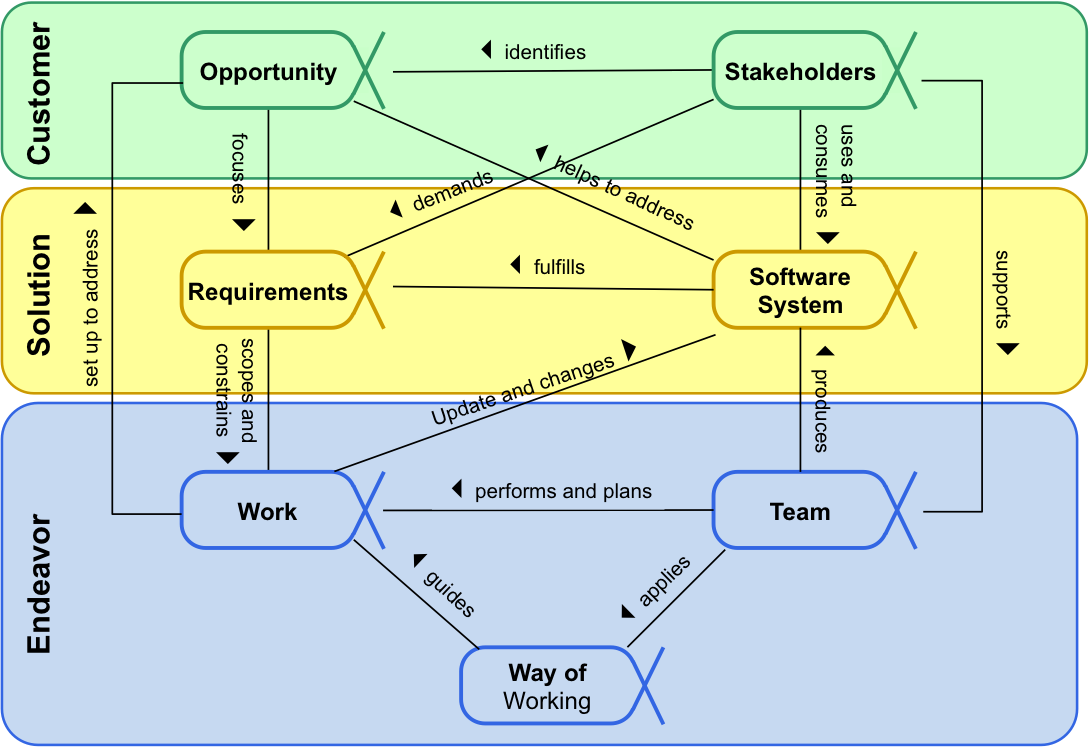
\includegraphics[width=0.8\textwidth]{img/prog}		
			\caption{Elementi di un progetto.}
		\end{figure} 
		
		
		\begin{figure}[H]
			\centering
			\subfloat[\underline{\hyperref[opportunity]{Opportunity}}.]{{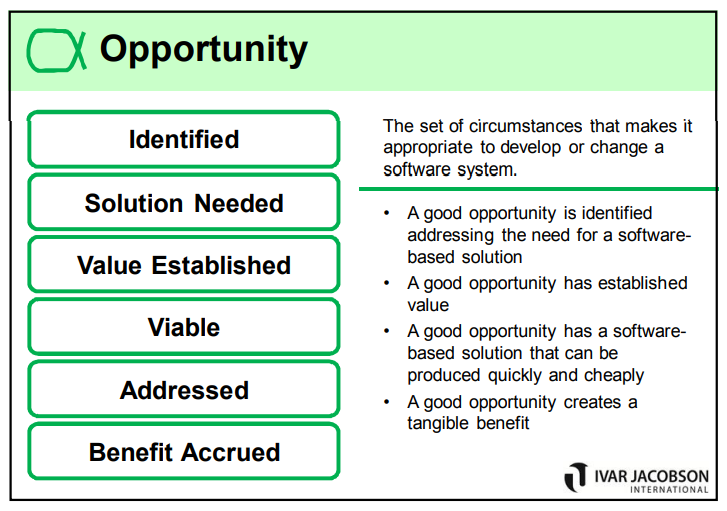
\includegraphics[width=0.46\textwidth]{img/cards/opp}	}}
			\qquad
			\subfloat[\underline{\hyperref[stakeholder]{Stakeholders}}.]{{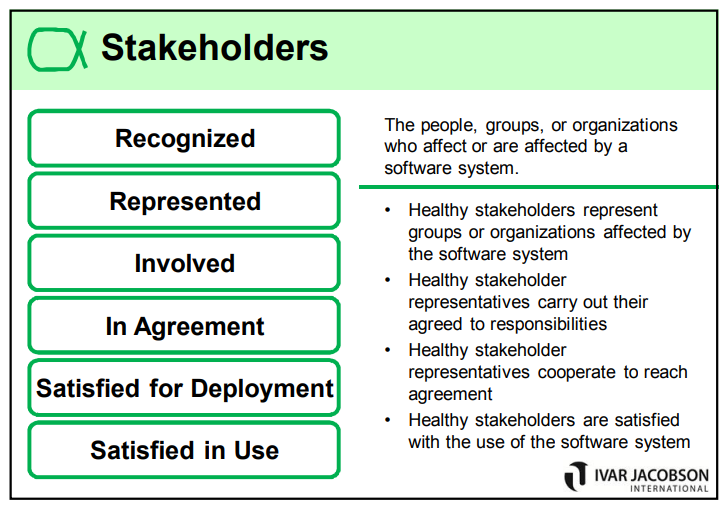
\includegraphics[width=0.46\textwidth]{img/cards/stake} }}
		\end{figure}
		
		\begin{figure}[H]
			\centering
			\subfloat[\underline{\hyperref[requirements]{Requirements}}.]{{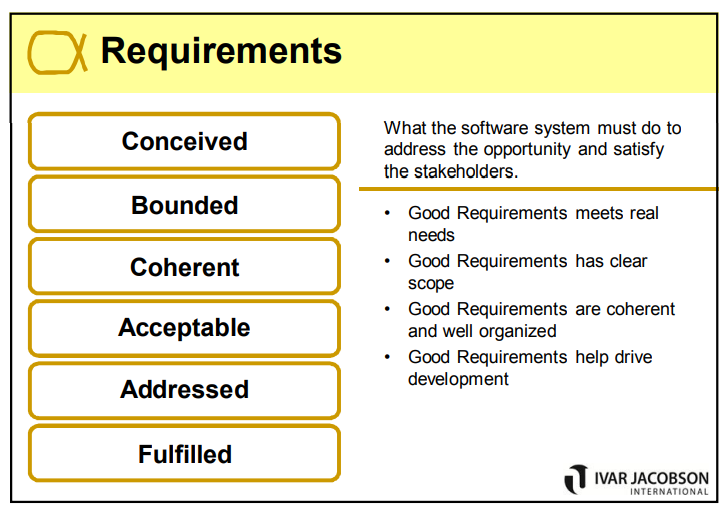
\includegraphics[width=0.46\textwidth]{img/cards/req}	}}		
			\qquad
			\subfloat[\underline{\hyperref[sistemasoftware]{Software System}}.]{{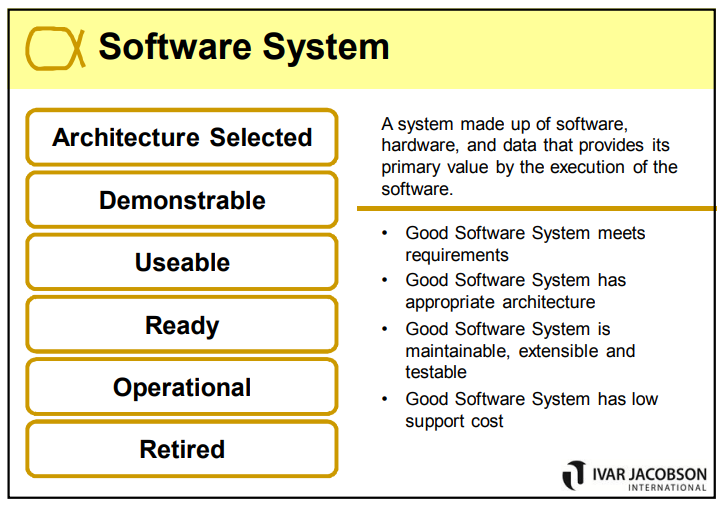
\includegraphics[width=0.46\textwidth]{img/cards/soft}	}}
		\end{figure} 
	
		\begin{figure}[H]
			\centering
			\subfloat[\underline{\hyperref[work]{Work}}.]{{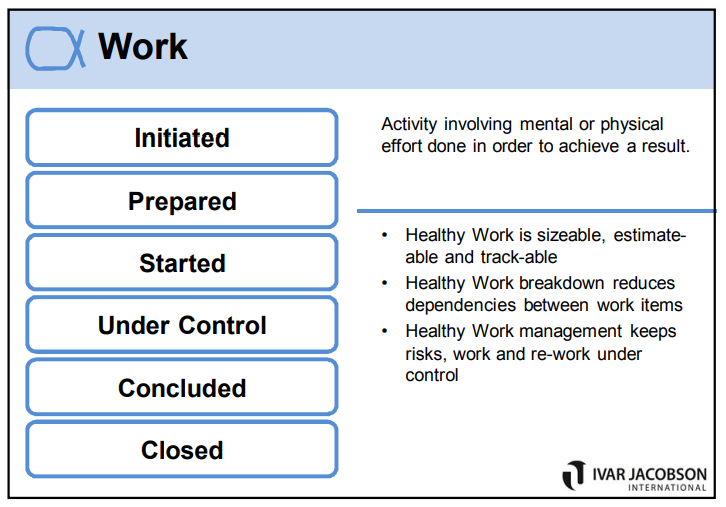
\includegraphics[width=0.46\textwidth]{img/cards/work}	}}		
			\qquad
			\subfloat[\underline{\hyperref[team]{Team}}.]{{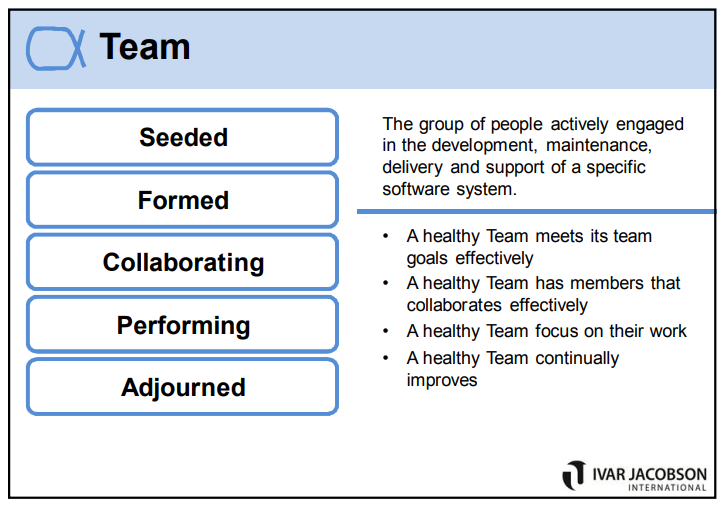
\includegraphics[width=0.46\textwidth]{img/cards/team}	}}
		\end{figure} 
	
		\begin{figure}[H]
			\centering
			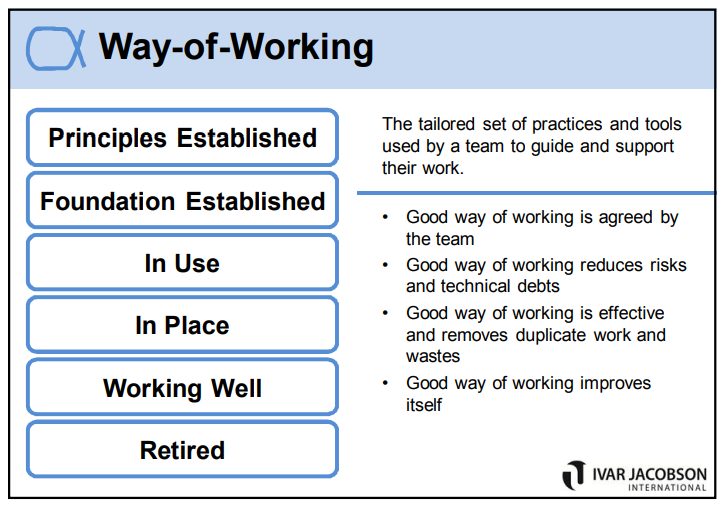
\includegraphics[width=0.46\textwidth]{img/cards/way}		
			\caption{\underline{\hyperref[way]{Way of working}}.}
		\end{figure} 
			
		Molto importante all'interno di un progetto è la \underline{\hyperref[gestioneprogetto]{Gestione di progetto}}. Per il progetto didattico vedi \underline{\hyperref[3p]{3P}}.
			
	%	\subsection{PROJECT-FIRST JUST-IN-TIME-PRINCIPLES APPROACH} \index{Project-first approach} \label{approach}
	%	Sfide maggiori se superate danno skills maggiori e maggior soddisfazione (ma non deve essere troppo alto e dare ansia, ma neanche troppo basso e annoiare).
		
		\subsection{PROGRAMMATORE} \index{Programmatore} \label{programmatore}
		È uno dei \underline{\hyperref[ruoli]{ruoli}} in un progetto. Sono la categoria più popolosa. Partecipano alla realizzazione e manutenzione del prodotto e hanno competenze tecniche, visione e responsabilità circoscritte.
		
		
		\subsection{PROGRAMMI VERIFICABILI}	\index{Programmi verificabili}	\label{programmiverificabili} %13 dicembre - verifica e validazione: analisi statica
		Serve dotarsi di uno standard di codifica coerente con le esigenze di \underline{\hyperref[verificare]{verifica}}. Per questo, per scrivere programmi verificabili, serve regolamentare l’uso del linguaggio di programmazione tramite principi da riflettere nelle Norme di Progetto:
		\begin{itemize}
			\item per assicurare \underline{\hyperref[comportamentopredicibile]{comportamento predicibile}};
			\item per usare \underline{\hyperref[criteriprog]{criteri di programmazione}} ben fondati;
			\item per \underline{\hyperref[pragmatico]{ragioni pragmatiche}};
		\end{itemize}
		Prima tecnica per essere sicuri: \underline{\hyperref[tracciamento]{tracciamento}}. \\
		Obblighi di analisi statica del codice: %slide 15/30
		\begin{itemize}
			\item \textbf{Analisi del flusso di controllo}: il modo in cui avanza il programma .%tramite il Program Counter?
			Alcune istruzioni cambiano il flusso (ad es: go to, cicli, ecc). Usare la ricorsione con grande parsimonia;
			\item\textbf{Analisi di flusso dei dati}: vedere l'ordine delle variabili. Si accerta che il programma non acceda a variabili prive di valore. Questa analisi è resa facile tramite incapsulazione. Non si fa eseguendo, ma prima. 
			\item \textbf{Analisi dei flusso d'informazione}: è il modo in cui valorizzo il dato. Determina la relazione tra ingressi e uscite di un'unità di codice. Bisogna capire se il valore informativo del dato è perso o meno.
			\item \textbf{Esecuzione simbolica}: dopo analisi di flusso di dati e d'informazione, so ora calcolare quale funzione dell'input produce l'output. L'uscita che vedo è la conseguenza di un flusso.
			\item \textbf{Verifica formale del codice}: usare le pre-condizioni e le post-condizioni e gli invarianti. Importante per vedere se il programma è corretto \textit{\underline{\hyperref[byconstruction]{by construction}}}; provare quindi la correttezza del codice sorgente rispetto alla specifica algebrica dei requisiti;
			\item \textbf{Analisi di limite}: limiti importanti sono overflow e underflow; rispetto dei limiti (fare \textit{range checking});
			\item \textbf{Analisi d'uso di stack}: Prima ragione di crescita: quando annido chiamate lo stack cresce. Lo stack è deciso all'elaborazione (quella è la massima estensione). Seconda ragione di crescita: i parametri che ci metto. Quando lo stack cresce oltre il suo confine cammina sull'heap, fare quindi attenzione che non tracimi [vedere le variabili del main dove stanno, se heap o stack];
			\item \textbf{Analisi temporale}: studiare le dipendenze temporali (latenza, tempestività) tra le uscite del programma e i suoi ingressi per verificare che il valore giusto sia prodotto al momento giusto;
			\item \textbf{Analisi d'interferenza}: mostrare l’assenza di effetti di interferenza tra parti isolate del sistema. Veicoli tipici di interferenza: memoria condivisa e I/O;
			\item \textbf{Analisi di codice oggetto}: assicurare che il codice oggetto da eseguire sia una traduzione corretta del codice e che non sia stata introdotta nessuna omissione dal compilatore;
		\end{itemize}
		
		
		\subsection{PROOF OF CONCEPT}	\index{Proof of Concept} \label{poc}
		Poc: risposta alle domande sulla fattibilità  della tecnologia selezionata. Prima di tutto capisco le domande e poi elaboro le risposte. Dimostro poi che il lavoro si può fare (rappresenta una \underline{\hyperref[baseline]{baseline}})e lo rendo accessibile al committente.
			
		\subsection{PROTOTIPO} \index{Prototipo} \label{prototipo}
		Dà l'idea di ció che sarà il \underline{\hyperref[prodotto]{prodotto}}. Serve per provare e scegliere possibili soluzioni. Può essere usato in modo \underline{\hyperref[incremento]{incrementale}} come la baseline, o "usa e getta" quindi \underline{\hyperref[iterazione]{iterativo}}).
		
		\subsection{PROVA}	\index{Prova}	\label{prova} %slide 13
		Una prove eseguibile è una procedura applicata a una \underline{\hyperref[testsuite]{batteria di prove}}.
	
	
